\section{Requisitos}

En esta sección se abordarán los requisitos planteados en el paquete, tanto los iniciales como los que se han ido planteando a lo largo del desarrollo ya sean funcionales o no funcionales. 

\subsection{Requisitos Funcionales}
\begin{itemize}
    \item RF1. Como usuario puedo utilizar el editor de diálogos para crear cajas y conexiones que representen conversaciones.
    \item RF2. Como usuario puedo exportar los diálogos de forma que sean legibles por el código del juego.
    \item RF3. Como usuario puedo reproducir los diálogos en el juego.
    \item RF4. Como usuario puedo añadir etiquetas al texto para reproducir animaciones del texto.
    \item RF5. Como usuario puedo utilizar el sistema de guardado para que mi juego tenga datos persistentes.
    \item RF6. Como usuario puedo usar el sistema de carga para cargar y descargar recursos.
    \item RF7. Como usuario puedo manejar los sonidos que aparecen en mi juego a través del sistema de sonido.
    \item RF8. Como usuario puedo añadir un sistema de niveles a mi juego mediante el sistema de experiencia.
    \item RF9. Como usuario puedo insertar un personaje jugable con cámara en cualquier perspectiva.
    \item RF10. Como usuario puedo insertar un personaje jugable con movimiento basado en físicas o discreto.
    \item RF11. Como usuario puedo insertar un personaje jugable ya sea en 2D o 3D.
    \item RF12. Como usuario puedo depurar las herramientas del paquete.
    \item RF13. Como usuario puedo generar una mazmorra o un laberinto usando el generador de mazmorras.
    \item RF14. Como usuario puedo utilizar algoritmos para encontrar el camino mínimo para salir de un laberinto o llegar a la hora de una mazmorra.
    \item RF15. Como usuario puedo modificar el tamaño y posición de una mazmorra.
    \item RF16. Como usuario puedo hacer que un objeto flote y rote.
    \item RF17. Como usuario puedo añadir interacciones a mi juego.
    \item RF18. Como usuario puedo añadir vida, daño y muerte a mi juego.
    \item RF19. Como usuario puedo añadir lanzar un objeto que utilice físicas en cualquier dirección.
    \item RF20. Como usuario puedo hacer que un objeto siempre mire a cámara.
    \item RF21. Como usuario puedo utilizar curvas de animación para sacudir la cámara en 2D y 3D, para cámaras de Unity y Cinemachine.
\end{itemize}

\subsection{Requisitos No Funcionales}

\begin{itemize}
    \item RNF1. Los módulos del paquete deben ser escalables.
    \item RNF2. Los módulos del paquete deben estar documentados.
    \item RNF3. El código del paquete debe ser legible y estar bien estructurado.
    \item RNF4. El paquete debe ser usable y recibir buenos resultados en las encestas de satisfacción.
\end{itemize}

\section{Herramientas y Tecnologías}

\subsection{C\# \& Unity}

Se ha utilizado Unity\cite{unity} como motor para el que está diseñado el paquete y C\#\cite{csharp} como lenguaje de programación, se ha elegido este motor dado que era el motor público más utilizado por estudiantes y equipos pequeños y medianos.

\subsection{Visual Studio}

Visual Studio\cite{visualstudio} es un IDE y editor de código para C++ y .Net y C\#, es el editor de código por defecto de Unity y el que se ha utilizado por defecto para el desarrollo del proyecto. 

\subsection{Git \& Github}

Github\cite{github} es un entorno de desarrollo colaborativo y control de versiones web basado en la tecnología Git. Para mantener el proyecto y poder trabajar en el desde distintos equipos, se ha alojado el proyecto de del paquete\cite{Repo} en él.

\subsection{UniTask}

UniTask\cite{UniTask} es una librería que ofrece una implementación de async/await sin necesidad de alocataciones de memoria basada en estructuras. Se ha aprovechado esta librería para la implementación del sistema de carga de escenas, ya que permite un funcionamiento asíncrono.

\section{Arquitectura y Análisis}
En la siguiente sección se detallan los detalles técnicos acerca del paquete, explicando los detalles de implementación de las distintas secciones, módulos y componentes.

\subsection{Sistema de Diálogos}
El sistema de diálogos está compuesto de tres subsistemas que hacen posible el renderizado de diálogo siguiendo los requisitos funcionales del proyecto. Estas tres partes son
el sistema de editor de diálogos (Figura \ref{fig:dialogueEditorExample}) (incluyendo la lógica que exporta el contenido de un diálogo a un asset que se pueda abrir), el sistema que gestiona la lógica de pintar el 
diálogo en el juego y el sistema que gestiona las animaciones del texto.

El código del editor es en parte el más complejo, ya que hace uso de la herramienta de Grafos de Unity para poder definir clases para los nodos del editor como muestra la 
Figura \ref{fig:nodos} se ha creado una clase específica por cada tipo de nodo ('Single Choice' y 'Multiple Choice'), también otra para los grupos que permiten agrupar distintos 
diálogos. También ha sido necesario crear clases para las ventanas nuevas, la del editor de diálogo, el 'GraphView' y la ventana de búsqueda.

El código de editor también se constituye de la lógica para convertir los nodos, grupos y conexiones (Figura \ref{fig:dialogueUml1}) a 'ScriptableObjects' que puedan guardarse en la memoria del dipositivo. Todo esto se gestiona mediante la clase
DialogueSystemIO (Figura \ref{fig:dialogueUml2}), que con sus funciones permite guardar, cargar y eliminar assets de tipo 'DialogueGraph'.  

\begin{figure}[H]
  \centering
    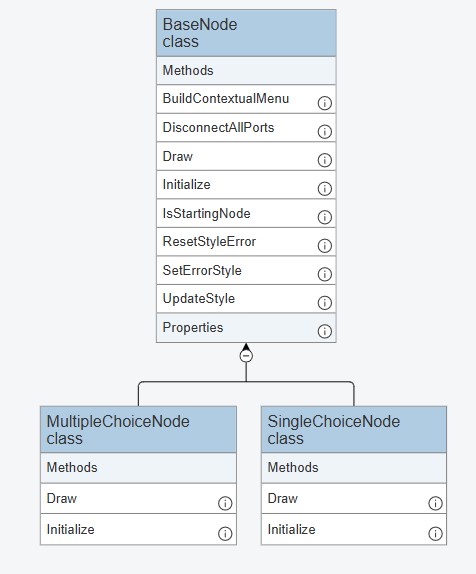
\includegraphics[width=350px,clip=true]{Node_Herencia.png}
  \caption{Diagrama de Herencia de Nodos del Sistema de Dialogo}
  \label{fig:nodos}
\end{figure}

\begin{figure}[H]
  \centering
    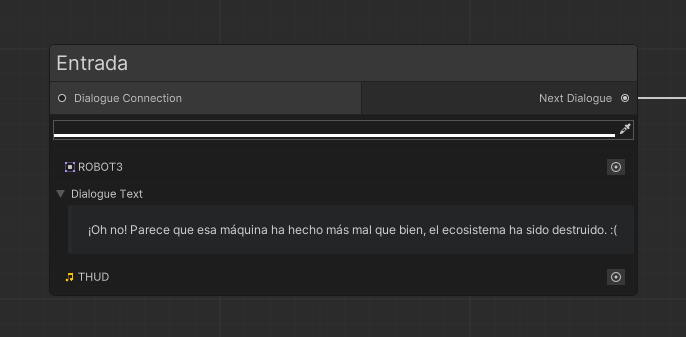
\includegraphics[width=350px,clip=true]{dialogue.png}
  \caption{Ejemplo del Editor del Sistema de Diálogo en uso}
  \label{fig:dialogueEditorExample}
\end{figure}

\begin{figure}[H]
  \centering
    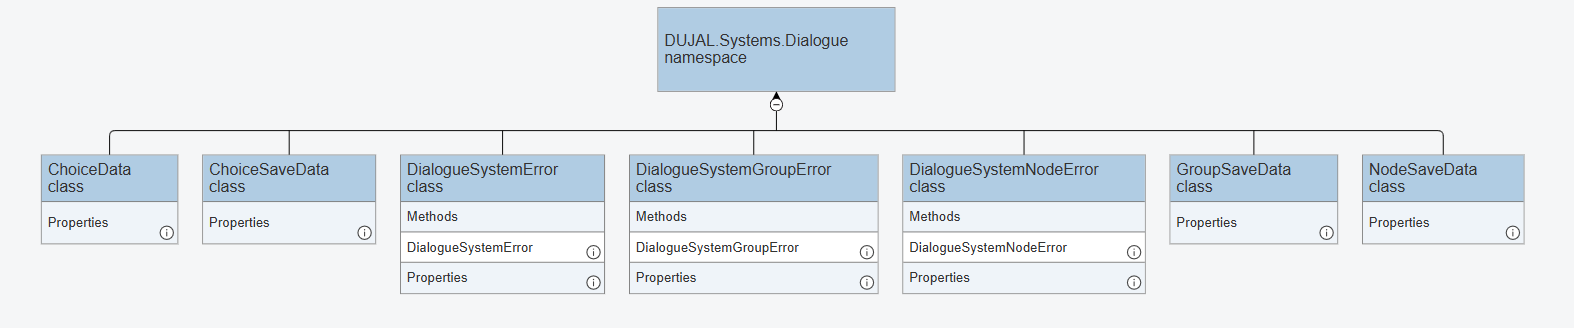
\includegraphics[width=500px,clip=true]{Dialogue_UML.png}
  \caption{Diagrama de Clases del Editor de Diálogos}
  \label{fig:dialogueUml1}
\end{figure}

\begin{figure}[H]
  \centering
    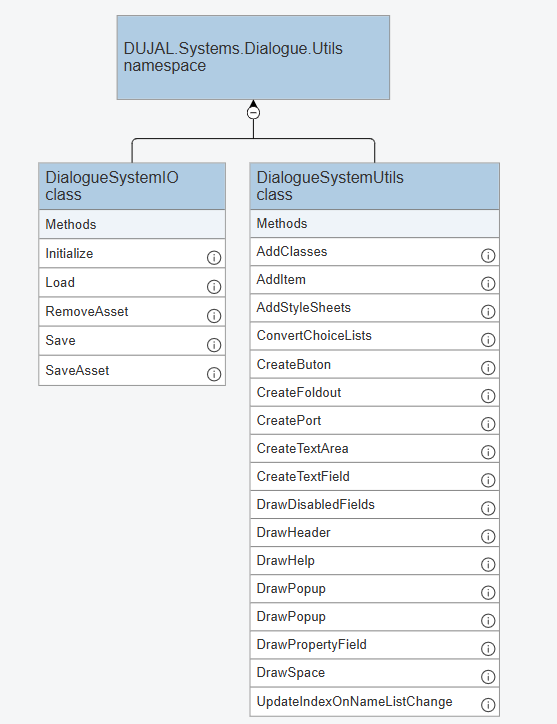
\includegraphics[width=350px,clip=true]{Dialogue_System_Utils.png}
  \caption{Diagrama de Clases Utils del Sistema de Diálogo}
  \label{fig:dialogueUml2}
\end{figure}

El sistema de dialogos de juego está compuesto por una clase de tipo Singleton que permite comenzar la reproducción del diálogo, elegir el diálogo concreto que se va a reproducir (El asset de tipo DialogueGraph que 
se quiere usar y el diálogo en concreto por el que se quiere comenzar la conversación) y configurar la reproducción de diálogo seleccionando cosas como la velocidad del texto, si se reproduce automáticamente, si se 
muesta todo el texto instantáneamente o se muestra en estilo 'Typewriter' etc. La gestión lógica de los diálogos se hace mediante un sencillo sistema de input en la que, mediante teclas, botones o el ratón, el el usuario
puede indicar que desea pasar al siguiente diálogo o elegir una opción concreta en el caso de que sea un nodo que permite ramificaciones. En lógica se selecciona la respuesta (0 - N) asociada al input que el usuario ha 
seleccionado. En el caso de los noos que no permiten elección múltiple, se selecciona por defecto siempre la opción cero, ya que siempre hay una sola. Esta parte del sistema también permite mostrar una imagen asociada 
a un interlocutor en concreto, o reproducir un sonido, utilizando el Sistema de Audio, asociado al interlocutor. El formato de sonido puede ser uno de tres tipos, en formato 'Gibberish' en la que se reproduce un 
sonido por cada letra mostrada en pantalla, en formato 'Unique Sound' en la que se reproduce un sonido por cada nueva caja de texto que se muestra, o en formato doblaje, en la que se reproducen las voces asociadas 
al texto mostrado. El resultado del sistema en uso se puede observar en la Figura \ref{fig:dialogueExample}.

\begin{figure}[H]
  \centering
    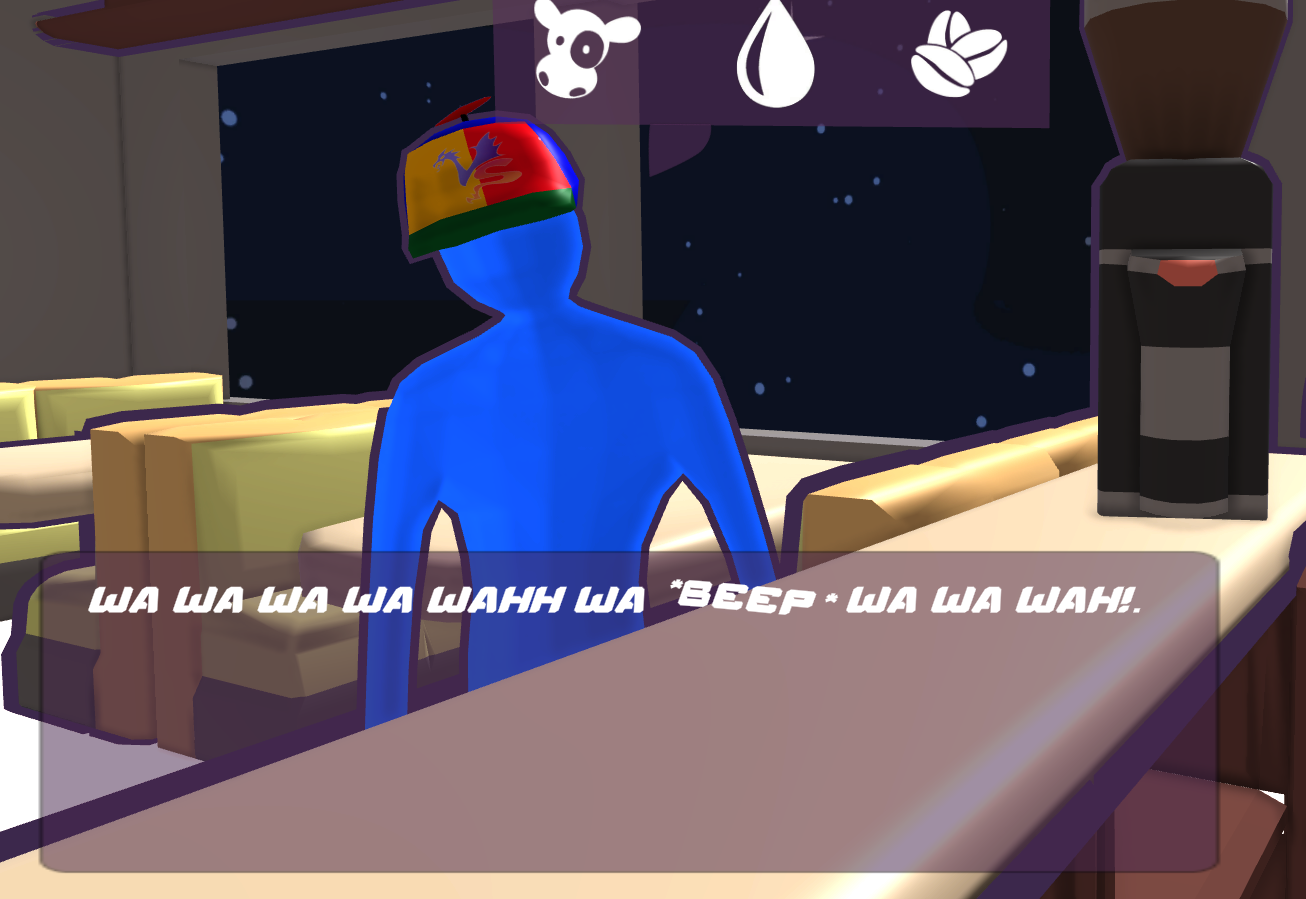
\includegraphics[width=350px,clip=true]{dialogueExample.png}
  \caption{Ejemplo del Sistema de Diálogo en uso}
  \label{fig:dialogueExample}
\end{figure}

El sistema de efectos de texto, que depende a su vez de la clase 'DialogueSystem', funciona con tags con formato '<>', el 'DialogueSystem' hace un pre-parsing del texto antes de mostrarlo al jugador para conseguir dos cosas:
en primer lugar borra las etiquetas pertinentes al 'TextEffectSystem' para que el texto se muestre como el diseñador pretendía, y, además, almacena en un mapa en el que se indican los índices del texto relevantes para aplicar 
el efecto, además de el efecto que se debe aplicar y sus modificadores. Cada efecto es gestionado por su propio tipo, dado que cada clase que hereda de TextEffect tiene sus propia implementación de 'UpdateEffect()',
tal y como se puede observar en la Figura \ref{fig:dialogueUml3}, que se utiliza mediante la Figura \ref{fig:dialogueUml4}. Lo más interesante referente al sistema de efectos de texto es que, al haber construido un
'template' la cual seguir para añadir efectos nuevos, y que el código interno y exclusivo de cada efecto es relativamente simple y pequeño, es muy sencillo escalar el sistem para añadir nuevos efectos. Una instancia
 del código de scripting mediante le cual se puede añadir un efecto nuevo se puede encontrar en el Código \ref{alg:wobbleAnimation}.

\begin{figure}[H]
  \centering
    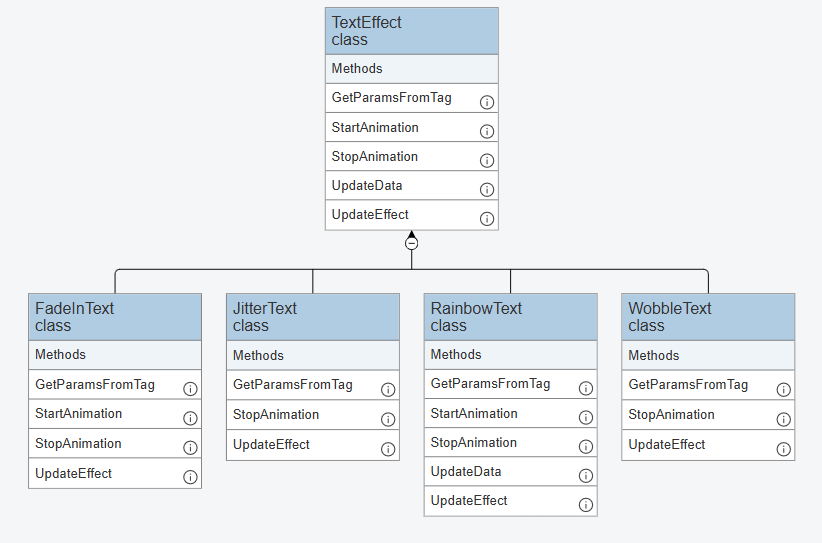
\includegraphics[width=350px,clip=true]{Text_Effects.png}
  \caption{Diagrama de Clases de Animaciones de Texto}
  \label{fig:dialogueUml3}
\end{figure}


\begin{figure}[H]
  \centering
    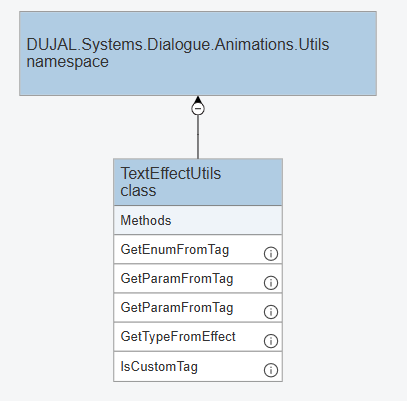
\includegraphics[width=350px,clip=true]{Text_Effect_Utils.png}
  \caption{Diagrama de Clases Utils del las Animaciones de Texto}
  \label{fig:dialogueUml4}
\end{figure}

\begin{mypython}[caption={Ejemplo de código utilizado para definir la animación de 'Wobble' en el texto.},label={alg:wobbleAnimation}]
    foreach (EffectInstance effect in effects) 
    {
        for (int i = effect.TextStartIdx; i < effect.GetTextEndIndex(); ++i)
        {
            var charInfo = animationHandler.TextInfo.characterInfo[i];
            if (!charInfo.isVisible)
            {
                continue;
            }
            
            var meshInfo = animationHandler.TextInfo.meshInfo[charInfo.materialReferenceIndex];
            var verts = meshInfo.vertices;
            for (int j = 0; j < 4; ++j)
            {
                int vertexIdx = charInfo.vertexIndex + j;
                float newOrigY = Mathf.Sin(Time.time * _speed[effectIdx] + verts[vertexIdx].x * 0.01f) * _amplitude[effectIdx];
                verts[vertexIdx] = verts[vertexIdx] + new Vector3(0f, newOrigY, 0f);
            }
        }
        effectIdx++;
    }
\end{mypython}

\subsection{Sistema de Experiencia}
El sistema de experiencia es un pequeño conjunto de clases que permite definir una lista de niveles de 'minLevel' a 'maxLevel' dada una función lineal, cuadrática, cúbica o 
 parabólica, este sistema permite definir callbacks para eventos de subida de nivel, aumento de experiencia y llegada al nivel máximo. El sistema gestiona automáticamente las
 subidas y el aumento de experiencia y dispone de funciones de acceso para obtener los datos actualizados en cualquier momento dado.

El sistema también cuenta con la posibilidad de crear 'ScriptableObjects' de tipo 'ExperienceMobAsset', que permiten definir la cantidad de experiencia que proporciona un evento 
 concreto, para ejemplificarlo se puede asumir que se estaría hablando de derrotar un enemigo en un juego de rol tradicional. El sistema cuenta con un manager singleton que 
 permite calcular el valor de la experiencia que daría un evento o 'Mob' concreto, además cuenta con la funcionalidad para definir distintos tipos de contextos modificadores 
 de experiencia.


\subsection{Sistema de Audio}
El sistema de audio o Audio Manager en código es una clase de tipo Singleton que permite definir una serie de 'ScriptableObjects' de tipo 'Sound'. Estos permiten a su vez que 
se les asigne un clip de audio y una serie de parámetros como si es un efecto de sonido o una canción, un modificador de volumen, de tono o si se desea que dicho sonido 
se reproduzca en bucle. La clase Audio Manager contiene a su vez un array de 'Sounds' y es capaz de reproducir, pausar, parar o reanudar cualquier sonido o canción que contenga. 
La clase tiene también la capacidad de gestionar una lista de música aleatoria de ambiente para ese tipo de juegos. El sistema tiene capacidad para separar los distintos tipos de 
sonido, música o efecto, en distintas pistas de audio con el fin de poder ajustar los dsitintos volúmenes por separado.    

\subsection{Sistema de Guardado}
El sistema de guardado está compuesto por tres clases llamadas: 'SaveDataHandler', 'SaveDataFileHandler' y 'SaveData'. 'SaveDataHandler' es una clase de tipo Singleton que 
sirve como API para gestionar las llamadas al guardado, creación de nuevos archivos de guardado u operaciones de borrado y copia de estos. El 'SaveDataFileHandler' es por 
otra parte el encargado de gestionar la conversión de datos en memoria dinámica a archivos .json almacenados en memoria estática del dispositivo. La clase 'SaveData' por últimos
es la clase en la que se almacenan los datos que se quieran guardar. El sistema soporta guardar tipos de datos alfanuméricos, listas y diccionarios de tipo 
'SerializableDictionary', dado que los diccionarios de C\# estándar no se pueden serializar a formato JSON. La implementación del 'SerializableDictionary' es muy sencilla, 
simplemente funciona como una lista de listas de tipo 'KeyValuePair', que a su vez contienen su respectiva clave y valor. Adicionalmente el sistema permite encriptar la 
partida guardada con una sencilla función de hash de XOR, de forma que no se almacene como texto en claro en el dispositivo.  

\begin{figure}[H]
  \centering
    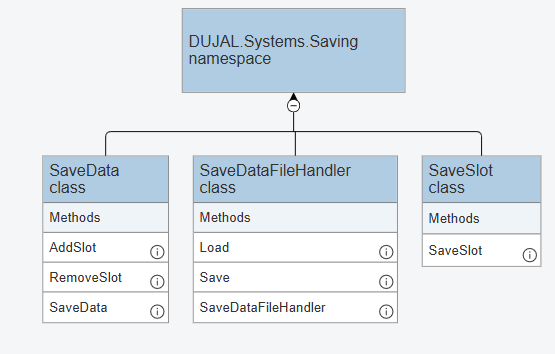
\includegraphics[width=350px,clip=true]{Saving.png}
  \caption{Diagrama de Clases del Sistema de Guardado}
  \label{fig:savinguml}
\end{figure}

\subsection{Sistema de Gestión Carga de Escenas}
El sistema de gestión de carga de escenas permite cargar de forma asíncrona y sustitutiva distntas escenas de un proyecto. El sistema automáticamente muestra una 
pantalla de carga que también esconde automáticamente una vez termina de cargar. La pantalla de carga puede mostrar opcionalmente el progreso de la carga. Añadir una nueva
 escena pasa, aparte de por añadir una nueva escena a las dependencias del proyecto en unity, por añadir un nuevo valor al enumerado de la clase 'SceneIndex'. Dicha clase 
 permite operar con 'SceneIndex' intercambiablemente como objetos, enumerados o enteros.

\subsection{Herramienta de Dibujado de Colisiones 2D}
La herramienta de dibujado de colisiones 2D (Figura \ref{fig:debug2d}), permite dibujar los colliders 2D de unity en builds empaquetadas del juego mediante el uso de
 'Line Renderers'. 

\begin{figure}[H]
  \centering
    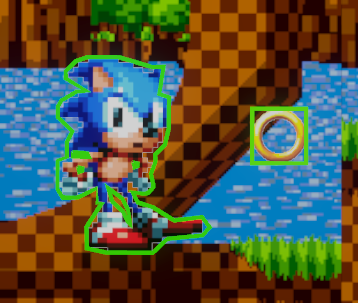
\includegraphics[width=350px,clip=true]{debug2d.png}
  \caption{Herramienta de Dibujado de Colisiones 2D en el modo 'Play' de Unity}
  \label{fig:debug2d}
\end{figure}

\begin{mypython}[caption={Algoritmo para pintar un box collider 2D.},label={alg:debugbox2d}]
    void HighlightCollider()
    {
        Vector3[] pos = new Vector3[4];
        pos[0] = transform.TransformPoint(new Vector3(_boxCol.size.x / 2.0f, _boxCol.size.y / 2.0f, 0));
        pos[1] = transform.TransformPoint(new Vector3(-_boxCol.size.x / 2.0f, _boxCol.size.y / 2.0f, 0));
        pos[2] = transform.TransformPoint(new Vector3(-_boxCol.size.x / 2.0f, -_boxCol.size.y / 2.0f, 0));
        pos[3] = transform.TransformPoint(new Vector3(_boxCol.size.x / 2.0f, -_boxCol.size.y / 2.0f, 0));
        _line.SetPositions(pos);
    }
\end{mypython}

\subsection{Herramienta de Cuadrícula}
La herramienta de cuadrícula o 'SnapToGrid' es un componente de editor que se puede añadir a cualquier objeto con un componente transform. En la configuración del componente
 se pueden definir el tamaño y altura de los elementos de la cuadrícula. Una vez añadido y configurado, el transform de dicho objeto quedará anclado a una cuadrícula como 
 célula del tamaño configurado, como se puede ver en la Figura \ref{fig:snaptogrid}.

 \begin{figure}[H]
  \centering
    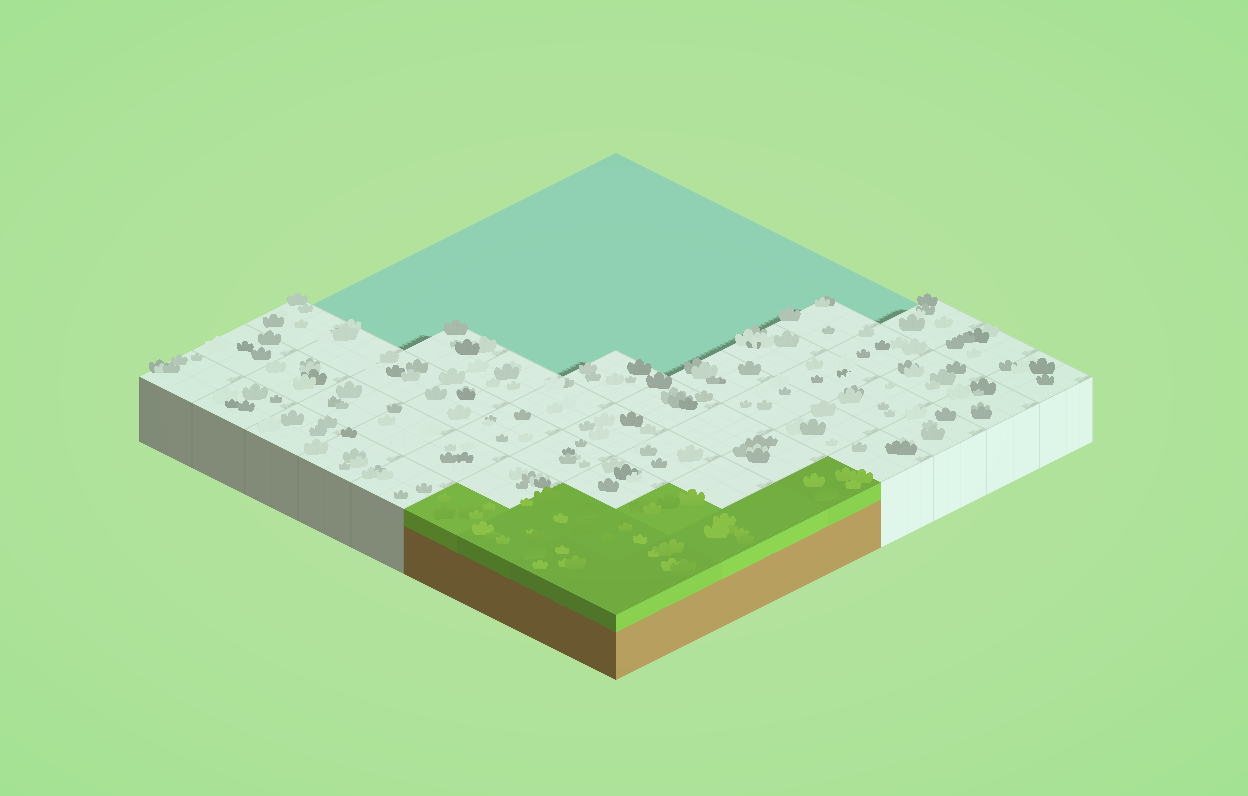
\includegraphics[width=350px,clip=true]{snaptogrid.png}
  \caption{Cuadrícula formada utilizando SnapToGrid}
  \label{fig:snaptogrid}
\end{figure}

\subsection{Generador de Mazmorras}
El generador de mazmorras está compuesto por dos componentes  que funcionan en tándem, por un lado existe la definición de tipos y algoritmos que permiten la construcción 
'teórica' de las mazmorras y laberintos, compuesto por clases y tipos como 'SquaredDungeon', 'Labyrinth' o 'Direction'. Estas clases (Figuras \ref{fig:dungen1} y \ref{fig:dungen2}) permiten generar una cuadrícula utilizando 
un array doble que posteriormente es poblado utilizando o bien el algoritmo de Prim (Código \ref{alg:dungenprim}) o Depth First Search, en adelante DFS (Código \ref{alg:dungendfs}). El sistema tiene la capacidad de transformar las matrices en grafos si es necesario, y es capaz de aplicarle a dichos grafos 
DFS o Breadth First Search para conseguir una lista de nodos en el orden indicado por el algoritmo.  

\begin{figure}[H]
  \centering
    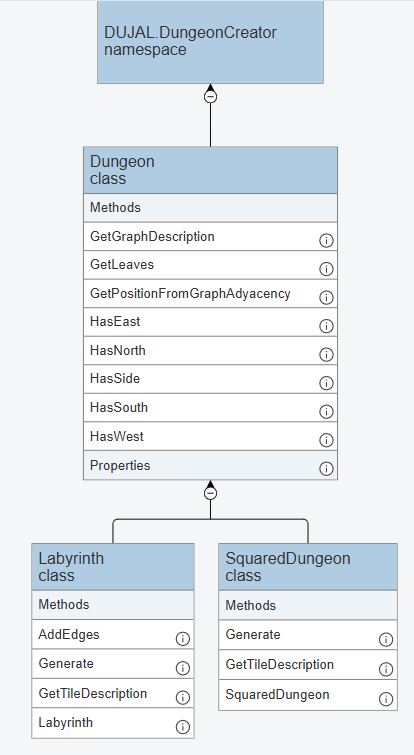
\includegraphics[width=200px,clip=true]{Dungeon_Generator.png}
  \caption{Diagrama Clases del Generador de Mazmorras}
  \label{fig:dungen1}
\end{figure}

\begin{figure}[H]
  \centering
    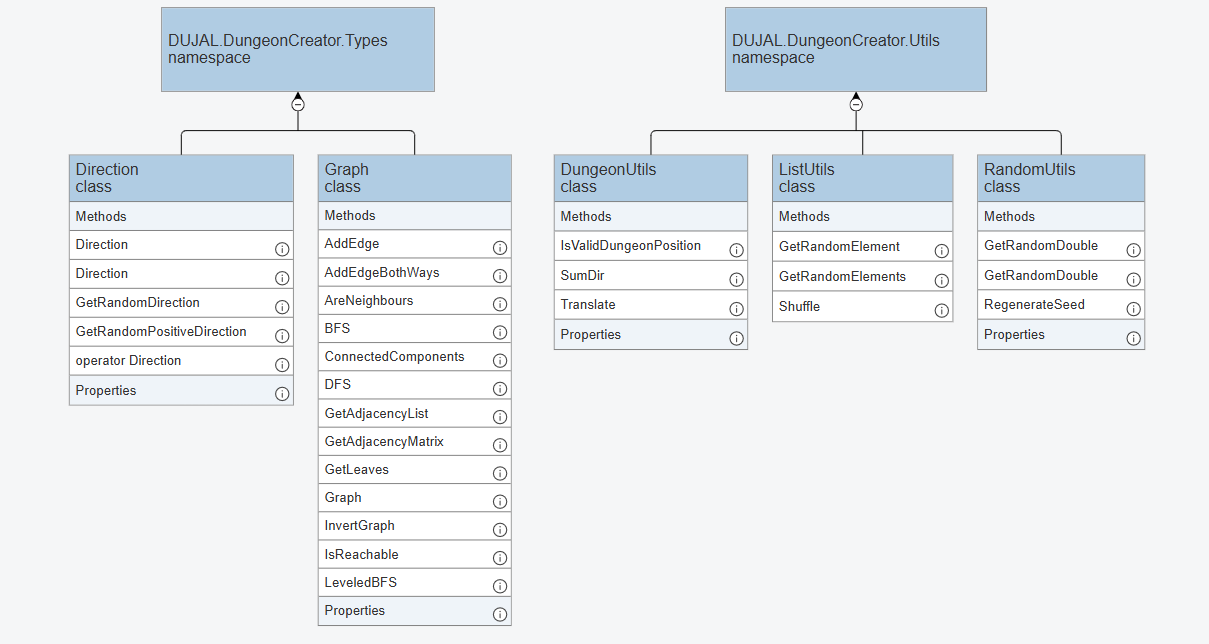
\includegraphics[width=450px,clip=true]{Dungeon_Generator_Utils.png}
  \caption{Diagrama Clases del Generador de Mazmorras}
  \label{fig:dungen2}
\end{figure}

\begin{mypython}[caption={Algoritmo de Generación de Mazmorras utilizando Prim.},label={alg:dungenprim}]
    protected void GeneratePrim(Vector2Int startingPos, int rooms = int.MaxValue)
    {
        PriorityQueue<Edge> edges = new();
        int num = 0;

        bool[,] visited = new bool[Size, Size];
        edges.Enqueue(new Edge(startingPos, startingPos + Direction.GetRandomPositiveDirection(), Random.Range(0, 10000)));
        edges.Enqueue(new Edge(startingPos, startingPos + Direction.GetRandomPositiveDirection(), Random.Range(0, 10000)));

        visited[startingPos.x, startingPos.y] = true;
        while (edges.Count() > 0 && num < rooms - 1)
        {

            Edge edge = edges.Dequeue();
            Vector2Int end = edge.end;
            Vector2Int origin = edge.origin;

            if (!visited[end.x, end.y])
            {
                visited[end.x, end.y] = true;
                _dungeonMatrix[end].Add(origin);
                _dungeonMatrix[origin].Add(end);
                ++num;

                for (Direction dir = 0; dir < Direction.Count; ++dir)
                {
                    Vector2Int newPos = end + dir.Vector;
                    if (DungeonUtils.IsValidDungeonPosition(newPos, Size))
                    {
                        edges.Enqueue(new Edge(end, newPos, Random.Range(0, 10000)));
                    }
                }
            }
        }
    }
\end{mypython}

\begin{mypython}[caption={Algoritmo de Generación de Mazmorras utilizando DFS.},label={alg:dungendfs}]
    protected void GenerateDFS(Vector2Int startingPos, int rooms = int.MaxValue)
    {
        int roomIdx = 0;
        Direction[,,] directionGrid = GenerateDFSDirectionGrid();

        bool[,] visited = new bool[Size, Size];

        Stack<int> roomStack = new();
        roomStack.Push(DungeonUtils.Translate(startingPos, Size));

        visited[startingPos.x, startingPos.y] = true;
        while (roomStack.Count > 0 && roomIdx < rooms)
        {
            Vector2Int roomPos = DungeonUtils.Translate(roomStack.Pop(), Size);
            for (Direction dir = 0; dir < Direction.Count; ++dir)
            {
                Vector2Int tentativePos = DungeonUtils.SumDir(directionGrid[roomPos.x, roomPos.y, dir], roomPos, Size);
                if (tentativePos != DungeonUtils.InvalidVector && !visited[tentativePos.x, tentativePos.y] && roomIdx < rooms)
                {
                    visited[tentativePos.x, tentativePos.y] = true;
                    roomStack.Push(DungeonUtils.Translate(tentativePos, Size));
                    _dungeonMatrix[roomPos].Add(tentativePos);
                    _dungeonMatrix[tentativePos].Add(roomPos);
                    ++roomIdx;
                }
            }
        }
    }
\end{mypython}

Una vez generada la mazmorra de forma teórica en formato mapa, es el turno de la parte dependiente del motor, que se encarga de instanciar 'GameObjects' de tipo 'DungeonRoom' 
basándose en la descripción de la matriz generada. Para ello la clase 'DungeonGenerator' tiene en si una lista de todas las permutaciones de sala posibles (Con puerta en cada 
posible lado entre norte, sur, este u oeste) y de todas los tipos de sala posibles (dados los tipos relevantes) para un juego o nivel concreto. Se busca una lista de 
'DungeonRooms' válidas para las coordenadas x, y que se quieran rellenar en un momento dado, y se selecciona una aleatoriamente para instanciar. Esto permite generar laberintos
y mazmorras como en los ejemplos de las Figuras \ref{fig:labyrinthExample} y \ref{fig:dungeonExample}.

\begin{figure}[H]
  \centering
    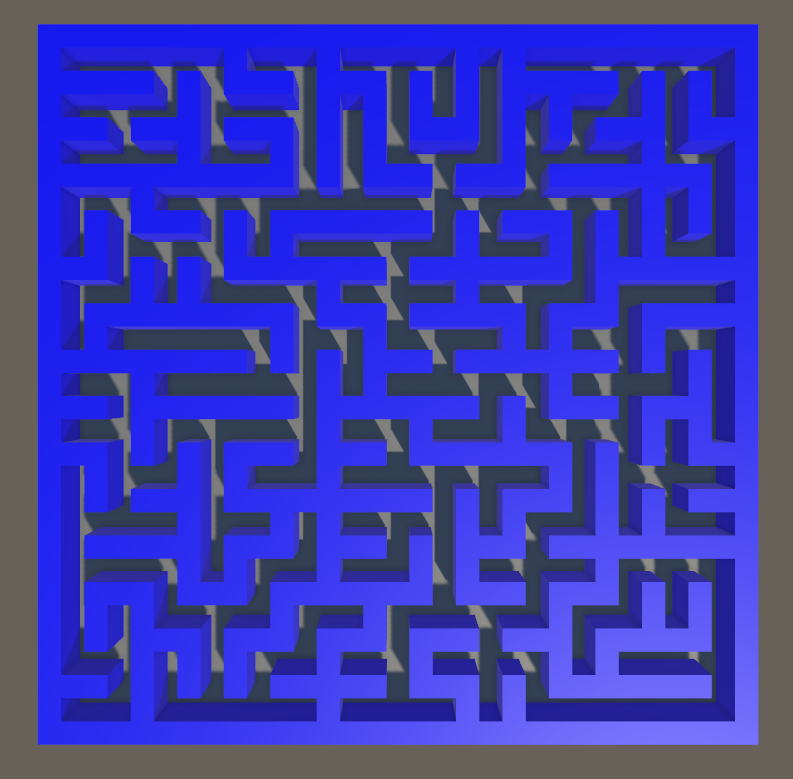
\includegraphics[width=350px,clip=true]{labyrinth_example.png}
  \caption{Laberinto Generado}
  \label{fig:labyrinthExample}
\end{figure}

\begin{figure}[H]
  \centering
    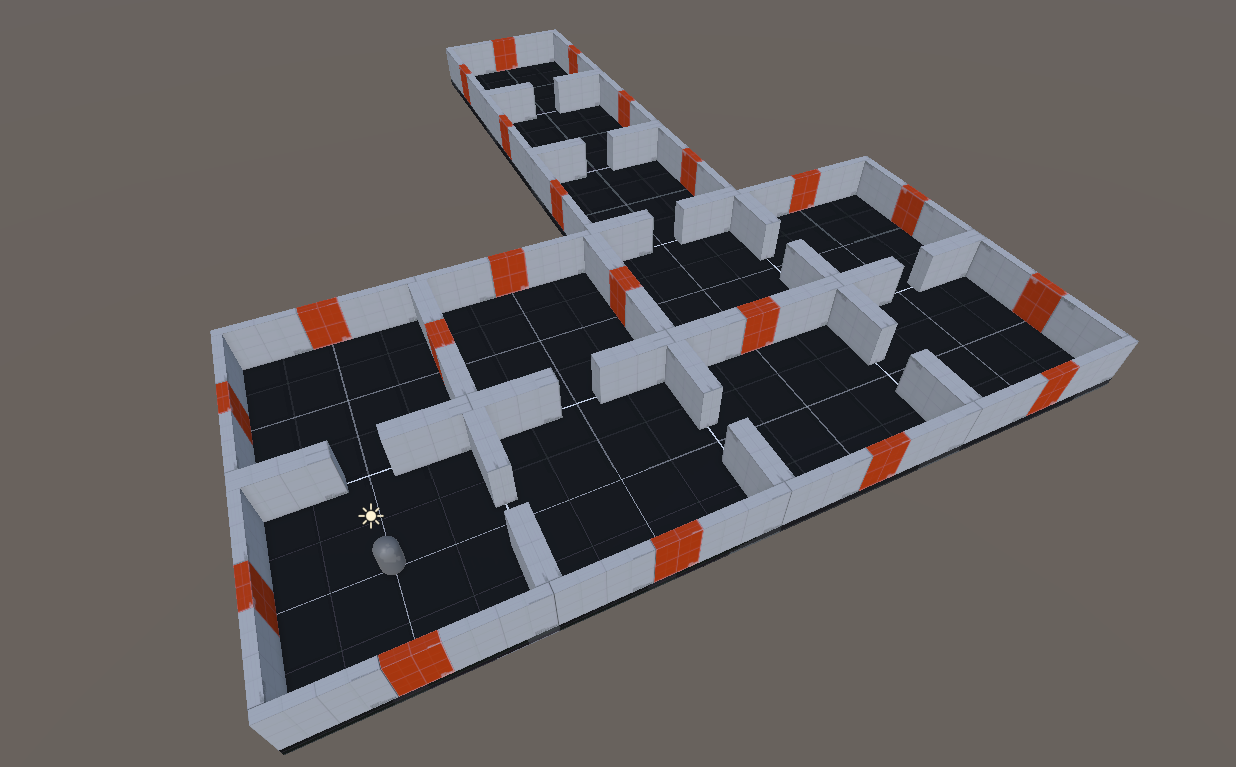
\includegraphics[width=350px,clip=true]{DungeonExample.png}
  \caption{Mazmorra Generada}
  \label{fig:dungeonExample}
\end{figure}

\subsection{Floater}
El componente de floater es una clase muy sencilla que permite darle a un objeto un movimiento de flotación sinuidal y de rotación constante dado un ángulo configurado. La 
implementación es muy sencilla dado que solo es necesario aplicarle un desplazamiento sinuidal en el bucle 'Update()' utilizando la diferencia de tiempo entre un ciclo y otro.

\begin{figure}[H]
  \centering
    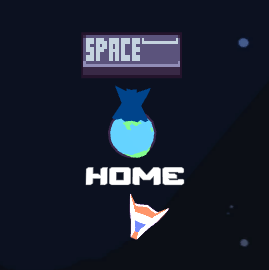
\includegraphics[width=200px,clip=true]{floaterExample.png}
  \caption{Ejemplo de uso de Floater, en el que el icono de 'Space' sube y baja para llamar la atención sobre el botón que debe presionar el jugador.}
  \label{fig:floaterExample}
\end{figure}


\subsection{Componente de Vida}
El componente de vida es un componente que se puede añadir a cualquier 'GameObject' y que permite atribuirle 'puntos de vida' a ese objeto. Aparte de métodos para acceder 
o modificar a la vida actual, también es posible añadir eventos para cuando el componente pierda vida, gane vida, cambie de vida, se quede sin vida o se cure completamente. 
Cabe destacar que el componente no es solamente útil para darle puntos de vida a un enemigo como se ha hecho tradicionalmente, sino que se podría utilizar, por ejemplo, 
para tener un callback concreto que disparar tras un temporizador, ya que podría deducirse un punto de vida por segundo.


\subsection{Componente de Interacción}
El componente de interacción permite añadir una callback a un 'UnityEvent' que se dispara cuando se pulsa el botón definido en el mapa de input correspondiente. 
Hay dos pares de clases 'Interactor', 2D y 3D, y dos pares de clases Interactable. Los interactors son las partes móviles, mientras que el interactable es el componente que 
tiene la callback asociada. Los interactables pueden configurarse para que solo se puedan usar una vez, se les puede configurar un radio de uso y se pueden deshabilitar. 
En el modo editor se puede pintar la esfera de radio que permite la interacción.

\subsection{LaunchRigidbody}
LaunchRigidbody es una clase pública y estática que no es un componente, al utilizar composición para funcionar no necesita existir en la escena, ya que recibe por parámetro 
el componente de Rigidbody que va a utilizar. La función además permite recibir dos 'Vector3' para indicar tanto la dirección como la potencia a la que se va a disparar el 
sólido rígido (Código \ref{alg:launchRigidbody}).

\begin{mypython}[caption={Funcionamiento de LaunchRigidbody.},label={alg:launchRigidbody}]
    public static void LaunchRigidBody3D(Rigidbody rigidbody, Vector3 launch, Vector3 power)
    {
        rigidbody.AddForce(new Vector3(launch.normalized.x * power.x, launch.normalized.y * power.y, launch.normalized.z * power.z), ForceMode.Impulse);
    }
\end{mypython}
    
\subsection{Componente de LookAtCamera}
Es un componente muy sencillo que rota un objeto en dirección a la 'Main Camera' (Código \ref{alg:alg:lookAtCamera}).

\begin{mypython}[caption={Funcionamiento de LookAtCamera.},label={alg:lookAtCamera}]
    var camera = Camera.main;
    transform.LookAt(transform.position + camera.transform.rotation * Vector3.forward, camera.transform.rotation * Vector3.up);
    transform.Rotate(_rotOffset);
\end{mypython}

\subsection{Componente de Sacudida de Cámara}
El componente de sacudida de cámara permite provocar un efecto de sacudida configurable de varias formas, aparte de definir la potencia y duración de la sacudida, se puede 
estipular que la intensidad de la sacudida varíe en el tiempo utilizando una curva de animación. Es relevante mencionar que hay dos variantes del componente, para cámaras 2D y 
cámaras 3D, como se menciona en la sección del estado del arte\ref{sec:estadodelarte}, en el estudio de Jump Trajectory\cite{Screenshake} se explica que la sacudida en 2D puede 
ser de traslación en los ejes XY ya que es como más se percibe el movimiento de la cámara en ese formato, pero que la sacudida en 3D debe ser por fuerza un movimiento 
exclusivamente rotatorio, ya que en caso contrario puede ocurrir clipping, además de que el movimiento de la cámara en esos casos es mucho más antinatural, ya que ninguna cámara
 en un espacio tridimensional puede trasladarse instantáneamente de esa forma. Cabe destacar también que el componente es capaz de funcionar con Cinemachine y cámaras normales. 

\subsection{Componentes de Movimiento}
Los componentes de movimiento del paquete están todos basados en un componente del que heredan, el 'MovementComponent' (Figura \ref{fig:umlMovimiento}). Este 'MovementComponent' 
es útil para gestionar funcionalidades base de todos los componentes de movimiento, como habilitar o deshabilitar los controles o contener la referencia al gestor y mapa de input, 
también gestiona el cambio de mando a teclado y ratón y vice versa.

\begin{figure}[H]
  \centering
    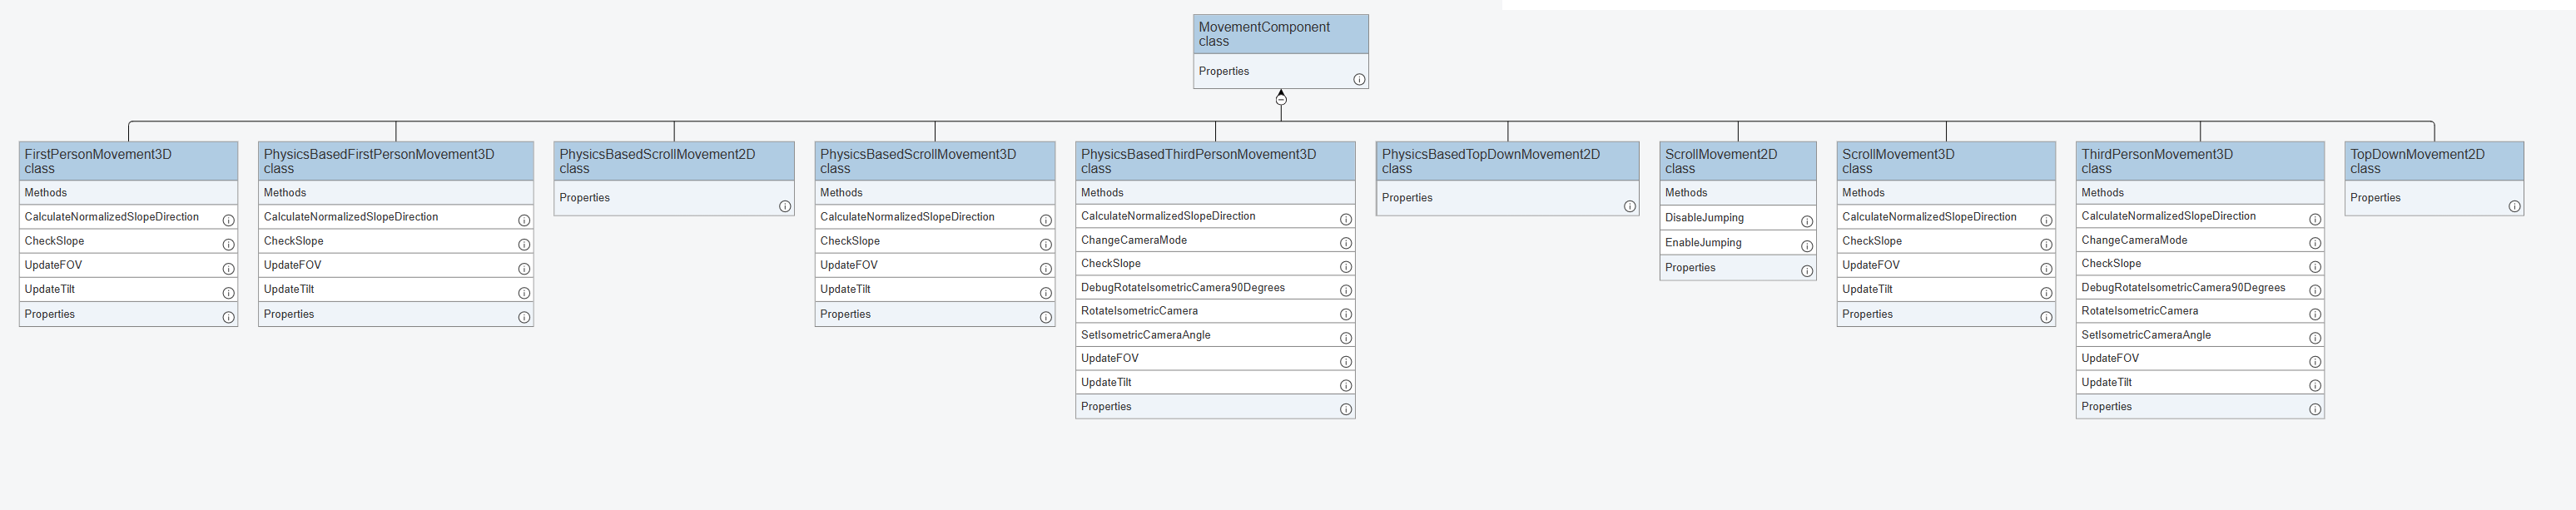
\includegraphics[width=350px,clip=true]{Movement.png}
  \caption{Diagrama de clases de los componentes de movimiento.}
  \label{fig:umlMovimiento}
\end{figure}

Aparte de los componentes de movimiento propios de cada cámara y si usan físicas o no, hay una clase 'CameraFollower' que gestiona las cámaras tridimensionales de Tercera Persona 
y Laterales. Esta clase gestiona sobre todo acompañar el movimiento del jugador, pudiendo configurarse para ajustar la suavidad con la que lo sigue, si alguno de los ejes 
es fijo, la zona muerta o si hay algún offset.

Otro dato relevante a nivel de arquitectura de software es que los componentes físicos se comportan como componentes auxiliares y externos, de forma que, por ejemplo,
 el PhysicsBasedFirstPersonMovement3D puede funcionar sin el componente de 'Wallrun' o el 'Dash', pero estos pueden añadirse al jugador tan solo con añadir el componente sin
 tener que hacer más ajustes.
 
Todos los componentes de movimiento funcionan con una máquina de estados que opera sobre el sólido rígido que constituye el cuerpo del jugador/personaje, y aplica distintas 
fuerzas a este dependiendo del input del jugador. El movimiento normal, por ejemplo, transforma el input de un joystick en dos ejes de \[-1,1\] a un vector director en el que 
aplicar la fuerza del movimiento. Por otra parte, agacharse implica forzar el estado a 'Crouching', bajar la cámara para ajustarse a la bajada de la cabeza del personaje, además de una reducción de velocidad y
un cambio en el FOV

\section{Niveles de Prueba}


\section{Documentación}
